\documentclass[journal]{IEEEtran}
% Supplementary material for SCooP-iT (RA-L multimedia attachment).
% Holds the floats that do not fit the 8-page limit of main.tex.
\usepackage{cite}
\usepackage{amsmath,amssymb,amsfonts}
\usepackage{graphicx}
\usepackage{xcolor}
\usepackage{tabularx}
\usepackage{multirow}
\usepackage{array}
\usepackage{booktabs}
\usepackage{siunitx}
\usepackage[hidelinks]{hyperref}
\graphicspath{{figures/}}
\newcommand{\todo}[1]{\textcolor{red}{[TODO: #1]}}
\newcommand{\unsure}[1]{\textcolor{orange}{[UNSURE: #1]}}
\newcommand{\Ttransform}[2]{\ensuremath{T_{\mathrm{#1}}^{\mathrm{#2}}}}
\newcommand{\cmark}{$\checkmark$}
\newcommand{\xmark}{--}
\renewcommand{\thetable}{S-\Roman{table}}
\renewcommand{\thefigure}{S\arabic{figure}}
\renewcommand{\thesection}{S\Roman{section}}

\begin{document}
\title{Supplementary Material for\\SCooP-iT: An Indoor Testbed for Collaborative Perception over Measured Wireless Links}
\author{Jorich Loquero and Ming-Chun Lee}
\maketitle

\section{Full Sensor Specification}
\begin{table*}[!t]
\caption{Per-Agent Sensor Specifications}
\begin{center}
\renewcommand{\arraystretch}{1.2}
\setlength{\tabcolsep}{4pt}
\scriptsize
\begin{tabular}{@{}p{2.0cm} p{2.6cm} p{5.6cm} p{1.9cm} p{2.1cm} p{1.5cm}@{}}
\toprule
\textbf{Equipment} & \textbf{Model Type} & \textbf{Characteristics} & \textbf{Resolution} & \textbf{FoV} & \textbf{Rate} \\
\midrule
\multicolumn{6}{@{}l}{\textit{Mobile Agents}} \\
LiDAR & Ouster OS1-64 & \texttt{mobile\_1}, 100 m range & 1024 $\times$ 64 & 45$^\circ$ vert. & 10 Hz \\
LiDAR & Ouster OS1-128 & \texttt{mobile\_2}, 100 m range & 1024 $\times$ 128 & 45$^\circ$ vert. & 10 Hz \\
Stereo Camera & ZED 2i & RGB stereo, baseline 120 mm & 1920 $\times$ 1080 & 110$^\circ$ $\times$ 70$^\circ$ & 30 Hz \\
 & & IMU 6-axis, barometer, magnetometer & -- & -- & 400 Hz \\
RGBD & RealSense D455 & RGB, global shutter & 1280 $\times$ 800 & 90$^\circ$ $\times$ 65$^\circ$ & 30 Hz \\
 & & Stereo IR, global shutter, baseline 95 mm & 1280 $\times$ 720 & 87$^\circ$ $\times$ 58$^\circ$ & 30 Hz \\
 & & IMU BMI 055 & -- & -- & 200 Hz \\
 Radar & TI IWR6843ISK & 60--62 GHz, 3 TX / 4 RX & \shortstack[l]{7.5\,cm range \\ $14.2^\circ$ az., $57^\circ$ el.} & $\pm$60$^\circ$ az., $\pm$20$^\circ$ el & 10 Hz \\
Radar & TI IWR6843ISK & 62--64 GHz, 3 TX / 4 RX & \shortstack[l]{7.5\,cm range \\ $13.8^\circ$ az., $55^\circ$ el.} & $\pm$60$^\circ$ az., $\pm$20$^\circ$ el & 10 Hz \\
Radar & TI MMWCAS-RF-EVM & 76--81 GHz, 4$\times$ AWR2243 cascade, 12 TX / 16 RX & \todo{--} & \todo{--} & \todo{--} Hz \\
CSI extractor & RPi 4B (BCM43455c0) & Nexmon, monitor mode, 80 MHz, 1 antenna & 256 subcarriers & -- & $\sim$100 Hz \\
Wi-Fi USB Dongle &  D-Link AX1800 & USB, 5 GHz 802.11ac; iw / iperf3 endpoint & -- & -- & 5/1 Hz \\
Computer &  MIC-713-OX4B2 & NVIDIA Jetson AGX Orin & -- & -- & -- \\

\midrule
\multicolumn{6}{@{}l}{\textit{Infrastructure Agents}} \\
RGB Camera & Arducam B0495 & AR0234, color global shutter, M12 lens & 1920 $\times$ 1200 & 95$^\circ$ diag. & 30 Hz \\
Radar & TI IWR6843ISK & 61.75--64 GHz, 3 TX / 4 RX & \shortstack[l]{7.5\,cm range \\ $13.9^\circ$ az., $56^\circ$ el.} & $\pm$60$^\circ$ az., , $\pm$20$^\circ$ & 10 Hz \\
CSI extractor & RPi 4B (BCM43455c0) & Nexmon, monitor mode, 80 MHz, 1 antenna & 256 subcarriers & -- & $\sim$100 Hz \\
Wi-Fi USB Dongle & Edimax N150 & USB, 5 GHz 802.11ac; iw / iperf3 endpoint & -- & -- &  5/1 Hz \\

\bottomrule
\end{tabular}
\end{center}
\label{tab:sensors}
\end{table*}


\section{Recorded Topics and Clock Statistics}
\begin{table*}[!t]
\caption{Recorded topics per unit (representative rates).}
\label{tab:topics}
\begin{center}
\renewcommand{\arraystretch}{1.2}
\setlength{\tabcolsep}{4pt}
\scriptsize
\begin{tabular}{@{}p{6.2cm} p{6.6cm} p{2.6cm}@{}}
\toprule
\textbf{Topic (namespace)} & \textbf{Message Type} & \textbf{Rate} \\
\midrule
\multicolumn{3}{@{}l}{\textit{\texttt{mobile\_1/}}} \\
\texttt{ouster/lidar\_packets} & \texttt{ouster\_sensor\_msgs/PacketMsg} & 640 Hz \\
\texttt{ouster/imu\_packets} & \texttt{ouster\_sensor\_msgs/PacketMsg} & 100 Hz \\
\texttt{ouster/metadata} & \texttt{std\_msgs/String} & latched \\
\texttt{radar\{1,2\}/radar/points\_all} & \texttt{PointCloud2} & 10 Hz \\
\texttt{zed/left/image\_rect\_color} & \texttt{Image} (+\,\texttt{CameraInfo}) & 15 Hz \\
\texttt{zed/depth/depth\_registered} & \texttt{Image} & 15 Hz \\
\texttt{zed/imu/data}, \texttt{zed/imu/mag} & \texttt{Imu}, \texttt{MagneticField} & 200 / 50 Hz \\
\texttt{zed/odom}, \texttt{zed/pose}, \texttt{zed/path\_*} & \texttt{Odometry}, \texttt{PoseStamped}, \texttt{Path} & 15 Hz \\
\texttt{tf}, \texttt{tf\_static} & \texttt{TFMessage} & --- \\
\addlinespace
\multicolumn{3}{@{}l}{\textit{\texttt{mobile\_2/}}} \\
\texttt{color/image\_raw} & \texttt{Image} (+\,\texttt{CameraInfo}) & 30 Hz \\
\texttt{depth/image\_rect\_raw} & \texttt{Image} (+\,\texttt{CameraInfo}) & 30 Hz \\
\texttt{infra\{1,2\}/image\_rect\_raw} & \texttt{Image} (+\,\texttt{CameraInfo}) & 30 Hz \\
\texttt{extrinsics/depth\_to\_infra\{1,2\}} & \texttt{realsense2\_camera\_msgs/Extrinsics} & latched \\
\texttt{imu} & \texttt{Imu} & 200 Hz \\
\texttt{visual\_slam/tracking/*}, \texttt{status} & \texttt{Odometry}, \texttt{PoseStamped}, \texttt{Path} & 30 Hz \\
\addlinespace
\multicolumn{3}{@{}l}{\textit{\texttt{infra\_N/}}} \\
\texttt{image\_raw} & \texttt{Image} (+\,\texttt{CameraInfo}) & 30 Hz \\
\texttt{radar/points\_all} & \texttt{PointCloud2} & 10 Hz \\
\addlinespace
\multicolumn{3}{@{}l}{\textit{\texttt{sniffer/}}} \\
\texttt{csi} & \unsure{\texttt{csi\_msgs/Csi}} & $\sim$100--140 Hz \\
\addlinespace
\multicolumn{3}{@{}l}{\textit{All units}} \\
\texttt{wifi/status} & \texttt{wifi\_monitor\_msgs/WifiLinkStatus} & 5 Hz \\
\texttt{wifi/iperf}, \texttt{wifi/iperf\_r2r} & \texttt{wifi\_monitor\_msgs/IperfResult} & per test \\
\texttt{ntp/status}, \texttt{ntp/events} & \texttt{ntp\_monitor\_msgs/NtpStatus}, \texttt{String} & 10 Hz / event \\
\bottomrule
\end{tabular}
\end{center}
\end{table*}

\begin{table}[t]
\centering
\caption{Clock synchronization across all sequences (server:
\texttt{mobile\_1}). 
\todo{Values from a single live pass; update once all sequences are processed.}}
\label{tab:ntp}
\footnotesize
\begin{tabular}{@{}lccccc@{}}
\toprule
& \multicolumn{2}{c}{RMS offset} & & & \\
\cmidrule(lr){2-3}
Client & Median & Max & Jitter (med.) & Path delay (med.) & Steps \\
\midrule
\texttt{mobile\_2} & \SI{10.9}{\micro\second} & \SI{10.9}{\micro\second} & \SI{227}{\micro\second} & \SI{4.2}{\milli\second}  & 0 \\
\texttt{infra\_1}  & \SI{42.5}{\micro\second} & \SI{42.5}{\micro\second} & \SI{175}{\micro\second} & \SI{4.1}{\milli\second}  & 0 \\
\texttt{sniffer}   & \SI{28.7}{\micro\second} & \SI{28.7}{\micro\second} & \SI{619}{\micro\second} & \SI{15.6}{\milli\second} & 0 \\
\bottomrule
\end{tabular}
\end{table}


\section{Reference Map and Error Distributions}
% Reference map: full method (supplementary). \input from supplementary.tex,
% section "Reference Map and Error Distributions". Code: scoop_pipeline/
% map_stages/02b_bundle_adjust.py (bundle adjustment), 01_build_map.py
% (fusion: tsdf), analysis/mapping/{map_quality,wall_build,compare_maps}.py,
% analysis/odom/compare_trajs.py (quality measures).

\subsection{Overview}
\label{sec:supp_refmap}
The reference is built from one mapping session of the LiDAR robot in five
steps: (i) the scans are placed with a trajectory, each point at its own
time; (ii) a LiDAR-inertial SLAM solution \cite{glim} gives the initial
trajectory; (iii) plane bundle adjustment moves all poses jointly until the
planar surfaces seen from several places are as thin as the scans allow;
(iv) the scans are fused into a truncated signed distance field (TSDF) and
the map is its zero-level surface, with moving objects removed; (v) the
fiducial boards are posed in the map (Eq.~(1) of the main paper). The
quality measures of Sec.~\ref{sec:supp_quality} are computed on the
intermediate and final products and never enter the estimation.

Notation: $T=(R,\mathbf t)\in SE(3)$ maps the LiDAR frame to the world,
$\mathbf x$ is a point in the LiDAR frame, $\mathrm{Exp}/\mathrm{Log}$ map
between $\mathbb R^3$ and $SO(3)$, $[\mathbf a]_\times$ is the
cross-product matrix, $\mathbf e_z$ the vertical.

\subsection{Scan Placement}
A sweep lasts \SI{0.1}{\second}; point $j$ is measured at $t_j$. Its world
position is $\mathbf p_j = T(t_j)\,\mathbf x_j$, with $T(t)$ interpolated
between trajectory poses (spherical linear interpolation of the rotation,
linear of the translation), evaluated at 100 time bins per sweep, so the
residual motion within a bin is below \SI{1}{\milli\metre} at walking speed.

\subsection{Plane Bundle Adjustment}
\paragraph{Keyframes} The scans of each \SI{1}{\second} are placed, with the
input trajectory, in the frame of their middle pose and thinned to
\SI{5}{\centi\metre}; the keyframe poses $T_k$, $k=1..K$, are the
unknowns, and the motion within a keyframe is kept from the input.

\paragraph{Planes} The keyframes' points are binned in world cubes of edge
$c=\SI{0.5}{\metre}$. With $\lambda_1\le\lambda_2\le\lambda_3$ the
eigenvalues of a cube's scatter matrix over its $N$ points and
$\sigma_i=\sqrt{\lambda_i/N}$, a cube is a plane when
$\sigma_1<\SI{6}{\centi\metre}$, $\sigma_1<0.3\,\sigma_2$,
$\sigma_2>0.1\,c$ and at least three keyframes see it. The thickness bound
is deliberately loose: a surface smeared by pose error must still qualify,
or the error it shows is never corrected.

\paragraph{Cost} For plane $f$ with unit normal $\mathbf n$ and offset $d$
($\mathbf n^\top\mathbf p=d$), the squared distances of all its points are
\begin{equation}
E_f=\sum_{k\in f}\sum_{j}\big(\mathbf n^\top(R_k\mathbf x_j+\mathbf t_k)-d\big)^2
   =\sum_{k\in f}\boldsymbol\pi_{kf}^\top C_{kf}\,\boldsymbol\pi_{kf},
\end{equation}
with the plane in the keyframe's frame and the keyframe's point cluster
\begin{equation}
\boldsymbol\pi_{kf}=\begin{bmatrix}R_k^\top\mathbf n\\ \mathbf n^\top\mathbf t_k-d\end{bmatrix},\qquad
C_{kf}=\sum_j\begin{bmatrix}\mathbf x_j\\1\end{bmatrix}\begin{bmatrix}\mathbf x_j\\1\end{bmatrix}^\top ,
\end{equation}
so the points themselves are not kept. For fixed poses the plane has a
closed form: $d=\mathbf n^\top\bar{\mathbf p}$ and $\mathbf n$ is the
eigenvector of the smallest eigenvalue of the world scatter matrix $S_f$,
so that
\begin{equation}
\min_{\mathbf n,d}E_f=\lambda_{\min}\big(S_f(T)\big),
\end{equation}
the plane's squared thickness summed over its points \cite{balm}. The
bundle adjustment minimizes
\begin{equation}
E(T)=\sum_f\lambda_{\min}\big(\tilde S_f(T)\big)+E_{\mathrm{odo}}+E_{g}+E_{0},
\label{eq:ba}
\end{equation}
where $\tilde S_f$ uses the weighted clusters
$\tilde C_{kf}=w_{kf}\,\tfrac{\min(N_{kf},n_{\mathrm{eff}})}{N_{kf}}\,C_{kf}/\sigma_p^2$:
$\sigma_p=\SI{2}{\centi\metre}$ is the point noise along the normal;
$n_{\mathrm{eff}}=30$ caps a keyframe's count, since its points share one
pose error; and $w_{kf}=\min(1,\delta/\rho_{kf})$ is a Huber weight on the
keyframe's RMS distance to the plane,
$\rho_{kf}=(\boldsymbol\pi^\top C\boldsymbol\pi/N)^{1/2}$, with
$\delta=\SI{5}{\centi\metre}$.

\paragraph{Priors} Directions that no plane observes (the length of a
corridor) keep the input's relative motion between consecutive keyframes,
\begin{equation}
\begin{aligned}
\mathbf e_R&=\mathrm{Log}\big(\Delta\bar R^\top R_k^\top R_{k+1}\big),\quad
\mathbf e_t=R_k^\top(\mathbf t_{k+1}-\mathbf t_k)-\Delta\bar{\mathbf t},\\
E_{\mathrm{odo}}&=\textstyle\sum_k \sigma_r^{-2}\|\mathbf e_R\|^2+\sigma_t^{-2}\|\mathbf e_t\|^2,
\end{aligned}
\end{equation}
with $\sigma_t=\SI{3}{\centi\metre}$ and $\sigma_r=0.3^\circ$ per keyframe.
Small floor cubes cannot see a slow vertical bend of the trajectory, so
each keyframe keeps the input's gravity direction,
$E_g=\sum_k\sigma_g^{-2}\|R_k^\top\mathbf e_z-\bar R_k^\top\mathbf e_z\|^2$,
$\sigma_g=0.1^\circ$, from the IMU through the SLAM solution. $E_0$ holds
the first keyframe fixed (the gauge); the boards later fix the frame.

\paragraph{Solver} Levenberg--Marquardt on right perturbations
$R\leftarrow R\,\mathrm{Exp}(\delta\boldsymbol\theta)$,
$\mathbf t\leftarrow\mathbf t+\delta\mathbf t$. With
$\mathbf m=R^\top\mathbf n$, the Jacobians of $\boldsymbol\pi$ are
$\partial\boldsymbol\pi/\partial\delta\boldsymbol\theta=[[\mathbf m]_\times;\mathbf 0^\top]$
and $\partial\boldsymbol\pi/\partial\delta\mathbf t=[0;\mathbf n^\top]$; the
plane parameters (two for the normal, one for the offset) are eliminated by
the Schur complement,
\begin{equation}
S=H_{pp}-\textstyle\sum_f H_{pf}H_{ff}^{-1}H_{fp},\qquad
(S+\mu\,\mathrm{diag}\,S)\,\delta\mathbf x=-\mathbf b ,
\end{equation}
a $6K\times6K$ system. After every step the planes are re-solved in closed
form, so the planes are always optimal for the current poses (variable
projection). Three rounds find the planes anew from the adjusted poses.

\paragraph{All poses} Each keyframe's correction
$\Delta T_k=T_k'T_k^{-1}$ is interpolated in time to every pose of the input,
$T'(t)=\Delta T(t)\,T(t)$, which keeps the motion within a keyframe.

\subsection{TSDF Fusion}
\paragraph{Why not the union} The usual map keeps one point per cell that
any scan hit. If the scans place a surface with a spread $\sigma$ along its
normal and a column of cells collects $M$ hits, a cell at offset $u$ holds
on average $M c\,\varphi(u/\sigma)/\sigma$ points and is kept once that
reaches about one, so the band extends to
\begin{equation}
u^\ast\approx\sigma\sqrt{2\ln\!\big(Mc/(\sqrt{2\pi}\,\sigma)\big)}\, ,
\end{equation}
which grows with every pass: a rarely hit cell counts as much as the dense
centre. On the 20261015 pass the union map's walls were
\SI{4}{\centi\metre} thicker than the scans that built it.

\paragraph{Fusion} A point $\mathbf p$ measured from sensor origin
$\mathbf o$ at range $r$ is a ray. Each cell $v$ (centre $\mathbf c_v$)
within $\pm\tau$ of the hit along the ray receives the projective signed
distance $d_v=r-\|\mathbf c_v-\mathbf o\|$ (positive in front of the
surface), and every ray's contribution is averaged
\cite{curless1996,vdbfusion}:
\begin{equation}
D(v)=\frac{\sum w\,d_v}{\sum w},\qquad W(v)=\sum w,\qquad w=1 .
\end{equation}
The weight is uniform: a weight that fades behind the hit makes the average
lopsided and moved a floor seen at grazing incidence \SI{8}{\milli\metre}
backwards in simulation. The surface is the zero crossing between
face-adjacent cells $a,b$ with $W\ge W_{\min}$ and $D_aD_b<0$,
$|D_a-D_b|<\tau$, placed at
$\mathbf c_a+\tfrac{D_a}{D_a-D_b}(\mathbf c_b-\mathbf c_a)$.

\paragraph{Parameters} Cell $c=\SI{2}{\centi\metre}$: the single-scan noise
on walls is $\sigma\approx\SI{1.2}{\centi\metre}$ and the point spacing at
\SIrange{3}{6}{\metre} is \SIrange{1.8}{3.7}{\centi\metre}, so finer cells
add no detail, and they would cost $8\times$ the memory. Truncation
$\tau=3\sigma_s$, with $\sigma_s$ the spread with which the scans place a
wall (Sec.~\ref{sec:supp_quality}, scans as placed with the reference
trajectory, whole run \SI{8.8}{\centi\metre},
$\sigma_s=8.8/3.29=\SI{2.7}{\centi\metre}$), giving
$\tau=\SI{8}{\centi\metre}$, at least three cells: a smaller
$\tau$ cuts off part of the spread before it is averaged, a larger one
distorts objects thinner than $\tau$. $W_{\min}=3$ rays.

\paragraph{Moving objects} Cells of a \SI{15}{\centi\metre} grid that rays
pass through in at least five scans while being occupied in others are
dynamic \cite{dufomap}, as are cells occupied for less than
\SI{1}{\second}; the surface points in them are removed.

\subsection{Quality Measures}
\label{sec:supp_quality}
\paragraph{Surface thickness} Around points sampled from the map,
\SI{0.25}{\metre} patches that are planar ($\sigma_3<0.6\,\sigma_2$) are
fitted with a plane, and the thickness is the 5--95\,\% spread of the
points' normal offsets, $3.29\sigma$ for a Gaussian spread; walls and floors
are reported separately. This is the mean-plane-variance idea of
\cite{razlaw} in a robust form. A patch whose offsets show an empty gap of
at least \SI{3}{\centi\metre} is split and each layer measured alone; it is
the two faces of a wall when the path passes on both sides, otherwise one
surface placed twice (a misalignment).

\paragraph{Scans as placed} At the same wall spots of the map, every scan
that saw a spot is placed with the trajectory under test, and the thickness
is measured for one scan, for the scans of \SI{1}{\second} to
\SI{300}{\second} around the spot's best view, and for the whole run. This
separates the sensor's noise floor, short-term pose error and drift from
the effect of the map's construction. With the reference trajectory:
\SI{4.6}{\centi\metre} for one scan, \SI{6.5}{\centi\metre} within
\SI{1}{\second}, \SI{8.8}{\centi\metre} over the whole run; with the SLAM
solution alone 4.9, 7.5 and \SI{19.2}{\centi\metre}. One scan differs
between trajectories only through deskewing.

\paragraph{Completeness} The share of a reference map's points with a point
of the map under test within \SI{10}{\centi\metre}, and the reverse
(accuracy), split by range from the path and height.

\paragraph{Board loop closure} The mapping session starts and ends at the
anchor board. The difference between the board's pose from the first and
the last sighting section measures the trajectory's accumulated error over
the run, against the detection noise within a section.

\paragraph{Trajectory error} Against the reference trajectory, the absolute
trajectory error (ATE) after the best rigid alignment and the relative pose
error (RPE) over \SI{1}{\second}, \SI{10}{\second} and \SI{100}{\second},
both as RMSE \cite{sturm2012}.

\paragraph{Timing} A pose stamped $\delta t$ away from its scans is turned
by $\omega\,\delta t$ at yaw rate $\omega$, so a trajectory's heading error
$e(t)$ against the reference is regressed on the reference's yaw rate (both
band-passed, \SIrange{0.3}{20}{\second}): the slope is $\delta t$, the
correlation tells whether the error is timing at all. Independently, the
IMU's $|\boldsymbol\omega|$ is lined up with a trajectory's (central
differences of its rotations), which gives the IMU's lag behind the LiDAR's
time, and pairs of scans are measured with the trajectory's stamps shifted,
which gives the shift that makes the scans agree best. On pass 20261015 the
SLAM trajectory's heading error follows the yaw rate ($r=0.92$,
$\delta t=\SI{46}{\milli\second}$), its scans agree best at
$+\SI{46}{\milli\second}$, and the IMU lags the LiDAR by
\SIrange{8}{14}{\milli\second}; running the SLAM with that IMU lag removed
leaves the \SI{46}{\milli\second}, so the offset is in the SLAM's output
poses and is corrected on export.

\paragraph{Independent starts} The bundle adjustment run from two different
input trajectories (the SLAM solution, and the same after scan-to-map
registration) should reach the same poses; their difference bounds how much
the result depends on its start: \SI{1.0}{\centi\metre} and $0.12^\circ$
ATE on pass 20261015; rebuilding it from the SLAM trajectory before and
after its \SI{46}{\milli\second} correction moves it by
\SI{0.5}{\centi\metre} and $0.10^\circ$.

\paragraph{Control distances} Laser-rangefinder distances between landmarks
fix the absolute scale, which none of the measures above observes.
\todo{Distances and errors.}

\subsection{Results, Mapping Pass 20261015}
% Reference construction, mapping pass 20261015 (mobile_2, 1387 s, 544 m).
% Read left to right: where a wall's spread comes from. Sources:
% analysis/mapping/wall_build.py (scans as placed at 300 wall spots; the
% reference's measured with the reference built before the 46 ms correction,
% traj_lidar_ba_glim_v1.txt), map_quality.py on each TSDF map (20,000
% sampled patches), odometry/mobile_2/*_loop_closure.json. Fusion rows: the
% poses of the BA started from scan-to-map (traj_lidar_ba.txt).
\begin{table}[!t]
\centering
\caption{Reference Construction, Stage by Stage (Pass 20261015)}
\label{tab:refmap_stages}
\footnotesize
\setlength{\tabcolsep}{2.5pt}
\begin{tabular}{lcccccc}
\toprule
Trajectory & \multicolumn{3}{c}{Walls, scans as placed} & \multicolumn{2}{c}{TSDF map} & Board loop \\
\cmidrule(lr){2-4}\cmidrule(lr){5-6}
 & 1 scan & 1\,s & run & walls / floors & doubled & closure \\
 & cm & cm & cm & cm & \% & mm / deg \\
\midrule
SLAM (GLIM)$^\ast$         & 4.9 & 7.5 & 19.2 & 14.3 / 3.6 & 2.0 & 10.8 / 1.24 \\
\textbf{SLAM + BA (ref.)}  & 4.6$^\S$ & 6.5$^\S$ & 8.8$^\S$ & \textbf{7.8 / 1.9} & 0.7 & 13.9 / 1.36 \\
\midrule
\multicolumn{7}{l}{\emph{Fusion, same scans and poses$^\dagger$}} \\
\quad union of points      & & & 8.4 & 12.5 / 3.6 & 0.3 & \\
\quad TSDF                 & & & 8.4 & 7.4 / 1.6  & 0.7 & \\
\bottomrule
\multicolumn{7}{l}{Left to right: the sensor (1 scan), short-term pose error (1\,s), drift}\\
\multicolumn{7}{l}{(run), fusion (map), the whole run's closure. Thickness: p95--p5 about}\\
\multicolumn{7}{l}{planes in 0.25\,m patches; median of 300 wall spots (scans as placed)}\\
\multicolumn{7}{l}{or of 20,000 sampled patches (map). Loop detection noise 6--8\,mm.}\\
\multicolumn{7}{l}{$^\ast$ as output, before its 46\,ms pose-time correction (Table~\ref{tab:glim_vs_ref}).}\\
\multicolumn{7}{l}{$^\S$ with the reference built before that correction (0.5\,cm ATE apart).}\\
\multicolumn{7}{l}{$^\dagger$ BA started from scan-to-map (1.0\,cm ATE from the reference); TSDF}\\
\multicolumn{7}{l}{\phantom{$^\dagger$} completeness 98\,\% of the union's surfaces.}
\end{tabular}
\end{table}

% Trajectories against the reference (SLAM + BA, traj_lidar_ba_glim.txt),
% pass 20261015. Source: check.py report (mapping_report_mapping_20261015.md).
% ATE after the best rigid fit; RMSE throughout.
\begin{table}[!t]
\centering
\caption{Trajectories Against the Reference (Pass 20261015)}
\label{tab:glim_vs_ref}
\footnotesize
\setlength{\tabcolsep}{2.5pt}
\begin{tabular}{lcccccc}
\toprule
Trajectory & \multicolumn{2}{c}{ATE} & \multicolumn{3}{c}{RPE, cm / deg} & Path \\
 & cm & deg & 1\,s & 10\,s & 100\,s & m \\
\midrule
SLAM (GLIM), as output      & 3.5 & 0.72 & 1.4 / 0.32 & 5.8 / 0.97 & 15.5 / 0.99 & 543.5 \\
+ pose-time correction      & 2.7 & 0.26 & 1.2 / 0.13 & 3.5 / 0.31 & 6.2 / 0.34  & 542.9 \\
+ scan-to-map$^\ast$        & 1.5 & 0.14 & 0.8 / 0.15 & 1.1 / 0.16 & 2.7 / 0.18  & 546.3 \\
\bottomrule
\multicolumn{7}{l}{Reference: SLAM + BA, path 543.6\,m.}\\
\multicolumn{7}{l}{$^\ast$ every scan registered to a map of the corrected SLAM poses: an}\\
\multicolumn{7}{l}{\phantom{$^\ast$} independent method, agreeing with the reference to 1.5\,cm.}
\end{tabular}
\end{table}


\begin{figure}[t]
\centering
\fbox{\parbox[c][4.5cm][c]{0.95\columnwidth}{\centering
\todo{Fig.: reference map colored by surface thickness (p95--p5), with
the fiducial boards, the control-distance endpoints, and the
second-pass trajectory overlaid. Distinct from the dataset paper's
reference-map render.}}}
\caption{Reference map colored by residual surface thickness, with the
fiducial network and control distances.}
\label{fig:refmap}
\end{figure}

\begin{figure}[t]
\centering
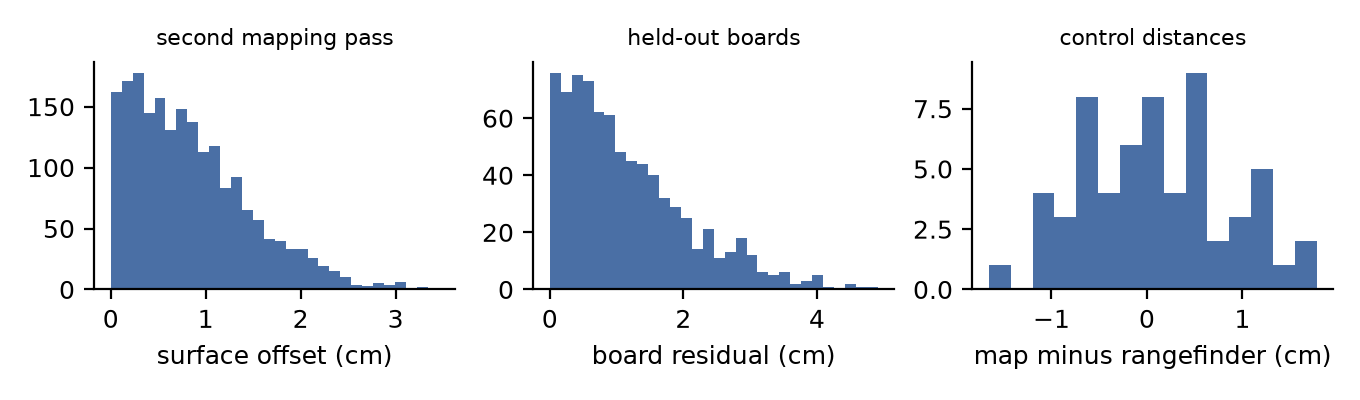
\includegraphics[width=\columnwidth]{figs/fig07_gt_errors.png}
\caption{Ground-truth error distributions from the three independent
checks. \todo{Dummy data.}}
\label{fig:gt_errors}
\end{figure}


\section{Post-Processing Data Flow}
\begin{figure*}[t]
\centering
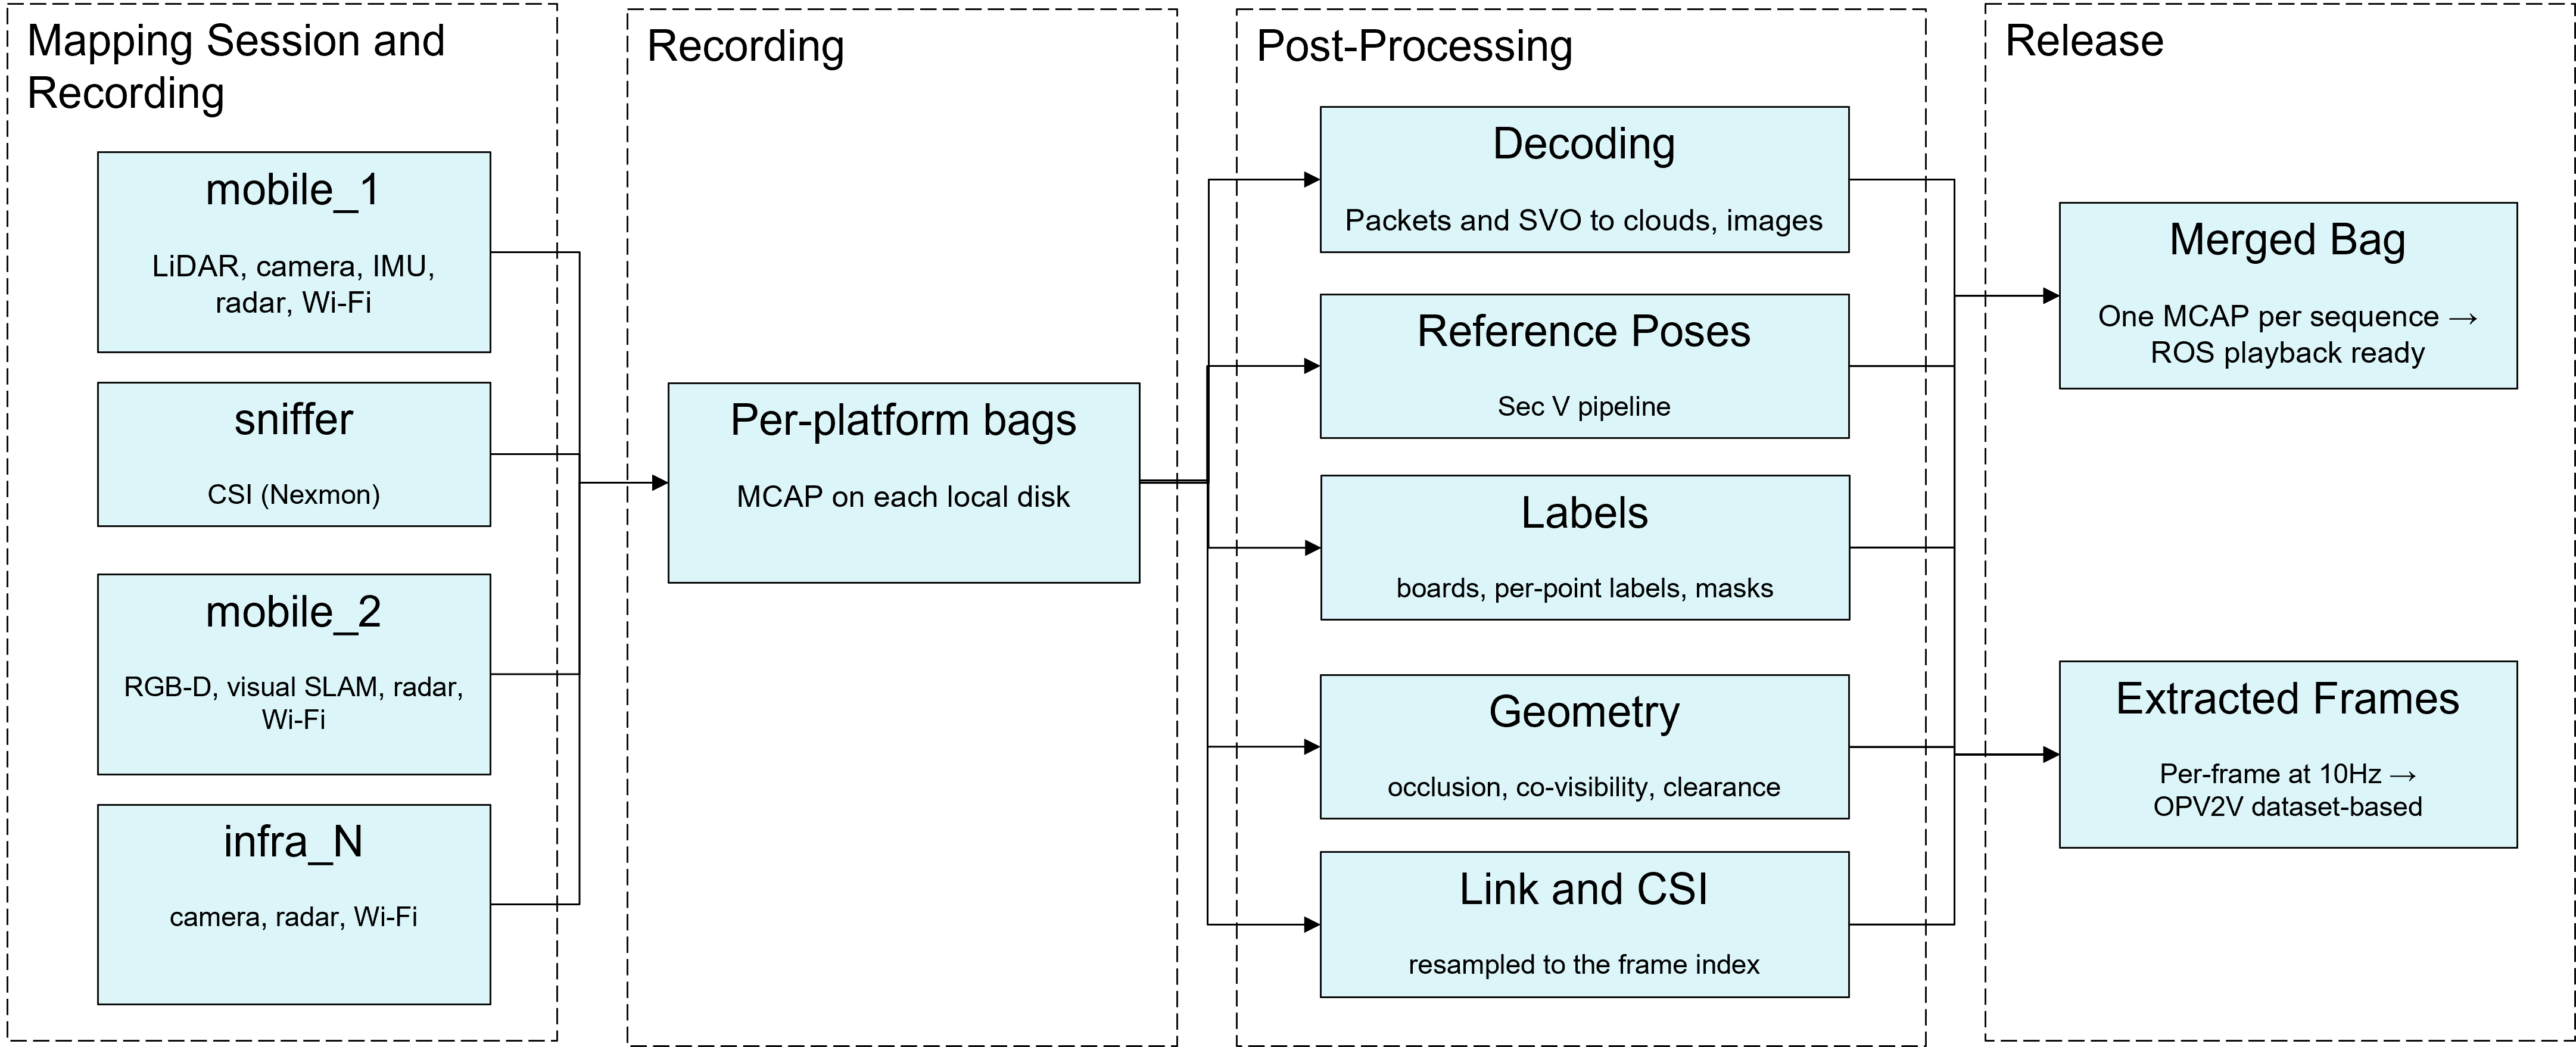
\includegraphics[width=\textwidth]{figs/fig03_dataflow.png}
\caption{Data flow from sensors to release files.}
\label{fig:dataflow}
\end{figure*}

\section{Sensor Intrinsics}
\todo{Per-sensor intrinsic parameters and the plots behind the
calibration table of the main paper: camera reprojection residual by
image region, LiDAR range bias by range, radar reflector offset by
range.}
%\begin{figure}[t]
\centering
\fbox{\parbox[c][4cm][c]{0.95\columnwidth}{\centering
\todo{Fig.~19: per-sensor intrinsic calibration plots.}}}
\caption{Intrinsic calibration residuals per sensor.}
\label{fig:app_intrinsics}
\end{figure}


\section{Per-Site Setup Effort}
\todo{Mapping-session length, number of boards, rangefinder distances,
software stack and versions, per site.}

\bibliographystyle{IEEEtran}
\bibliography{references}

\end{document}
